\documentclass[12pt]{article}
\usepackage[utf8]{inputenc}

\usepackage{enumitem}
\usepackage[margin=2cm]{geometry}

\usepackage{amsmath, amsfonts, amssymb}
\usepackage{graphicx}
\usepackage{tikz}
\usepackage{pgfplots}
\usepackage{multicol}

\usepackage{comment}
\usepackage{url}
\usepackage{calc}
\usepackage{subcaption}
\usepackage{circledsteps}
\usepackage{wrapfig}
\usepackage{array}

\setlength\parindent{0pt}

\usepackage{fancyhdr}
\pagestyle{fancy}
\fancyhf{}
\renewcommand{\headrulewidth}{2pt}
\renewcommand{\footrulewidth}{0pt}
\rfoot{\thepage}
\lhead{\textsc{Math} 244}
\chead{\textsc{Homework 9}}
\rhead{Fall 2023}

\pgfplotsset{compat=1.16}

% MATH commands
\newcommand{\ga}{\left\langle}
\newcommand{\da}{\right\rangle}
\newcommand{\oa}{\left\lbrace}
\newcommand{\fa}{\right\rbrace}
\newcommand{\oc}{\left[}
\newcommand{\fc}{\right]}
\newcommand{\op}{\left(}
\newcommand{\fp}{\right)}

\newcommand{\bi}{\mathbf{i}}
\newcommand{\bj}{\mathbf{j}}
\newcommand{\bk}{\mathbf{k}}
\newcommand{\bF}{\mathbf{F}}

\newcommand{\ra}{\rightarrow}
\newcommand{\Ra}{\Rightarrow}

\newcommand{\sech}{\mathrm{sech}\,}
\newcommand{\csch}{\mathrm{csch}\,}
\newcommand{\curl}{\mathrm{curl}\,}
\newcommand{\dive}{\mathrm{div}\,}

\newcommand{\ve}{\varepsilon}
\newcommand{\spc}{\vspace*{0.5cm}}

\DeclareMathOperator{\Ran}{Ran}
\DeclareMathOperator{\Dom}{Dom}

\newcommand{\exo}[3]{\noindent\textcolor{red}{\fbox{\textbf{Section {#1}, Problem {#2}}}\hrulefill   \textbf{({#3} Pts})}\vspace*{10pt}}

\begin{document}
\thispagestyle{empty}
	\noindent \hrulefill \newline
	MATH-244 \hfill Pierre-Olivier Paris{\'e}\newline
	Homework 10 Solutions \hfill Fall 2023\newline \vspace*{-0.7cm}
	
	\noindent\hrulefill
	
	\spc

	\exo{16.6}{2}{5}
	\\ 
	For the point $P$, we have $x = 1$, $y = 2$, $z=1$, so that
		\[
			\vec{r} (u, v) = \left\langle 1, 2, 1 \right\rangle \iff \left\lbrace \begin{matrix} 1 + u - v = 1 \\ 
			u + v^2 = 2 \\ 
			u^2 - v^2 = 1 . \end{matrix}\right. \iff \left\lbrace \begin{matrix} u - v = 0 \\ 
			u + v^2 = 2 \\ 
			u^2 - v^2 = 1 . \end{matrix}\right. 
		\]
	Notice that the third equation can be written as $(u - v)(u + v) = 1$. Using the first equation $u - v = 0$ and plugging that equation in the third, we see that for $\vec{r} (u, v) = \left\langle 1 , 2, 1 \right\rangle$, then $0 (u + v) = 1$ which is equivalent to $0 = 1$. This is impossible and therefore the point $P$ is not on the surface.

	For the point $Q$, we have $x = 2$, $y = 3$ and $z = 3$, so that
		\[
			\vec{r} (u, v) = \left\langle 2, 3, 3 \right\rangle \iff \left\lbrace \begin{matrix} 1 + u - v = 2 \\ 
			u + v^2 = 3 \\ 
			u^2 - v^2 = 3 . \end{matrix}\right. \iff \left\lbrace \begin{matrix} u - v = 1 \\ 
			u + v^2 = 3 \\ 
			(u-v)(u+ v) = 3 . \end{matrix}\right.
			\iff \left\lbrace \begin{matrix} u + v^2 = 3 \\ 
			u + v = 3 . \end{matrix}\right.
		\]
	Subtracting $u + v = 3$ from $u + v^2 = 3$, we get $v^2 - v = 0$. The solutions are $v = 0$ and $v = 1$. Therefore, $u = 3$ if $v = 0$ and $u = 2$ if $v = 1$. In this situation, we get
		\[
			\vec{r} (3, 0) = \left\langle 4, 3, 3 \right\rangle \neq \vec{OQ} \quad \text{ and } \quad \vec{r} (2, 1) = \left\langle 1, 2, 1 \right\rangle = \vec{OQ} .
		\]
	Therefore, since $\vec{r} (2, 1) = \vec{OQ}$, the point $Q$ lies on the surface.

	\spc 

	\exo{16.6}{4}{5}
	\\ 
	We have $y = u \cos v$ and $z = u \sin v$. Hence
		\[
			y^2 + z^2 = u^2 \cos^2 (v) + u^2 \sin^2(v) = u^2 = x .
		\]
	This is a paraboloid with the $x$-axis as its main axis.

	\spc 

	\exo{16.6}{10}{5}
	\\ 

	\begin{minipage}{0.5\textwidth}
	In the picture on the right, the line in green represents $u = \text{constant}$ and the lines in blue, $v = \text{constant}$. Here is the link to the Desmos app: \url{https://www.desmos.com/3d/8bb09174fc}.
	\vspace*{4cm} 
	\end{minipage}
	\begin{minipage}{0.5\textwidth}
	\begin{center}
	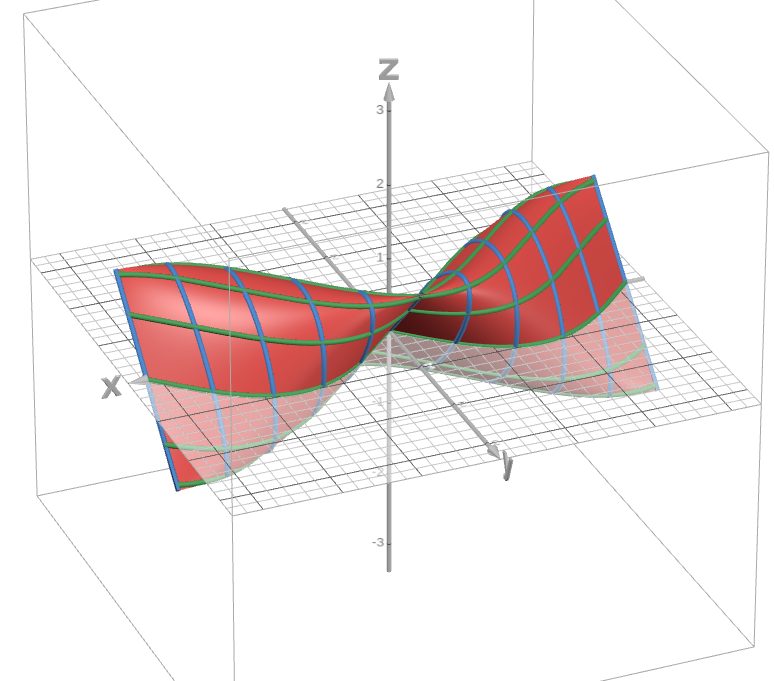
\includegraphics[scale=0.225]{figure1.png}
	\end{center}
	\end{minipage}

	\newpage

	\exo{16.6}{12}{5} 
	\\ 
	\begin{minipage}{0.5\textwidth}
	In the picture on the right, the line in green represents $u = \text{constant}$ and the lines in blue, $v = \text{constant}$. Here is the link to the Desmos app: \url{https://www.desmos.com/3d/67e0b4d314}.
	\vspace*{4cm} 
	\end{minipage}
	\begin{minipage}{0.5\textwidth}
	\begin{center}
	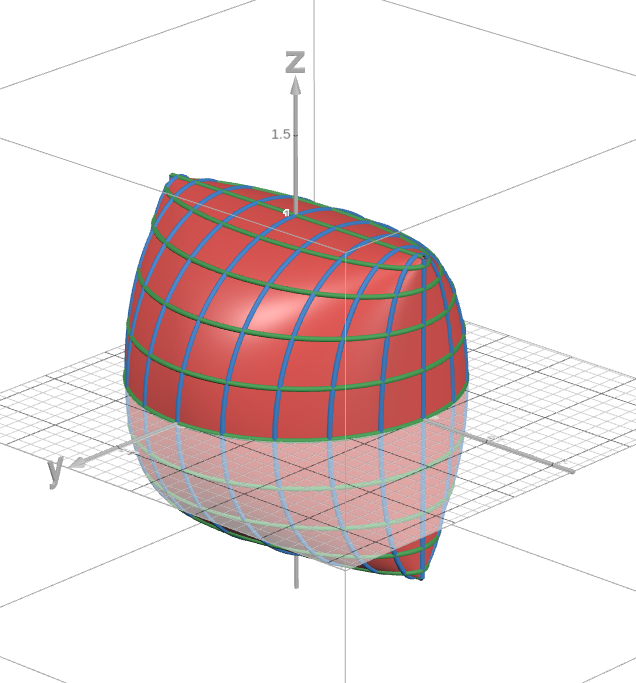
\includegraphics[scale=0.225]{problem12.png}
	\end{center}
	\end{minipage}

	\spc 

	\exo{16.6}{22}{5} 
	\\ 
	We put $x = v\cos u$ and $z = \frac{v}{\sqrt{3}} \sin u$. Since we want the part of the ellipsoid on the left of the $xz$-plane, we get from the equation of the ellipsoid:
		\[
			x^2 + 2y^2 + 3z^2 = 1 \iff y = -\sqrt{\frac{1 - x^2 - 3z^2}{2}} = - \sqrt{\frac{1 - v^2}{2}}
		\]
	Hence,
		\[
			\vec{r} (u, v) = (v \cos u , - (1/2) \sqrt{1 - v^2} , (v/\sqrt{3}) \sin (u)), 
		\]
	with $0 \leq u \leq 2 \pi$ and $0 \leq r \leq 1$. 

	\spc 

	\exo{16.6}{24}{5}
	\\ 
	Let $x = 3 \cos (u)$ and $z = 3 \sin (u)$. To make sure we get the part of the cylinder above the $xy$-plane, we let $u \in [0, \pi ]$. We also let $y = v$, with $-4 \leq v \leq 4$. Hence,
		\[
			\vec{r} (u, v) = (3\cos (u), v, 3 \sin (u)),
		\]
	with $0 \leq u \leq \pi$ and $-4 \leq v \leq 4$. 

	\spc 

	\exo{16.6}{42}{10}
	\\ 
	Here, we parametrize the cone using cartesian coordinates:
		\[
			\vec{r}(x, y) = \left\langle x, y, \sqrt{x^2 + y^2} \right\rangle .
		\]
	The region $D$ of interest is
		\[
			D = \{(x,y) \, : \, 0 \leq x \leq 1 , x^2 \leq y \leq x \} .
		\]
	We have
		\[
			\vec{r}_x \times \vec{r}_y = \begin{vmatrix} \vec{i} & \vec{j} & \vec{k} \\ 1 & 0 & \frac{x}{\sqrt{x^2 + y^2}} \\ 
			0 & 1 & \frac{y}{\sqrt{x^2 + y^2}} \end{vmatrix} = \left\langle \frac{-x}{\sqrt{x^2 + y^2}}, \frac{-y}{\sqrt{x^2 + y^2}} , 1 \right\rangle .
		\]
	Therefore,
		\[
			dS = \Big( \frac{x^2}{x^2 + y^2} + \frac{y^2}{x^2 + y^2} + 1\Big)^{1/2} = \sqrt{2} .
		\]
	Hence,
		\[
			\mathrm{Area} (S) = \iint_S \, dS = \iint_D \sqrt{2} \, dA = \int_0^1 \int_{x^2}^x \sqrt{2} \, dy dx = \sqrt{2} \int_0^1 x - x^2 \, dx = \frac{\sqrt{2}}{6} .
		\]

	\spc 

	\exo{16.6}{44}{10}
	\\ 
	A parametrization of the surface is
		\[
			\vec{r} (x, y) = \left\langle x, y, 4 - 2x^2 + y \right\rangle 
		\]
	where $0 \leq x \leq 1$ and $0 \leq y \leq x$. We then get
		\[
			\vec{r}_x \times \vec{r}_y = \begin{vmatrix} \vec{i} & \vec{j} & \vec{k} \\ 1 & 0 & -4x \\ 0 & 1 & 1 \end{vmatrix} = \left\langle 4x , -1, 1 \right\rangle 
		\]
	and so
		\[
			dS = \sqrt{2 + 16x^2} \, dA .
		\]
	Hence,
		\begin{align*}
			\mathrm{Area} (S) = \iint_D \sqrt{2 + 8x^2} \, dA &= \int_0^1 \int_0^x \sqrt{2 + 16x^2} \, dy dx \\ 
			&= \int_0^1 x \sqrt{2 + 16x^2} \, dx \\ 
			&= \frac{1}{16} \int_2^{18} \sqrt{u} \, du \\ 
			&= \frac{1}{48} \big( 18^{3/2} - 2^{3/2} \big) .
		\end{align*}
	
\end{document}


\exo{16.6}{46}{10}
	\\ 
	Notice that $z^2 = x - y$ and therefore $x - y \geq 0$ because $z^2 \geq 0$ for any value of $z$.
	Since $z$ is always positive, we can isolate $z$ form the equation
		\[
			x = z^2 + y \iff z = \sqrt{x - y} .
		\]
	Then, we parametrize the surface in the following way
		\[
			\vec{r} (x, y) = \left\langle x, y, \sqrt{x - y} \right\rangle ,
		\]
	with $D = \{ (x, y) \, : \, y \leq x \leq 1 , 0 \leq y \leq 2 \}$. 

	We have
		\[
			\vec{r}_x \times \vec{r}_y = \begin{vmatrix} \vec{i} & \vec{j} & \vec{k} \\ 1 & 0 & \frac{1}{2 \sqrt{x - y}} \\ 0 & 1 & \frac{-1}{\sqrt{x -y}} \end{vmatrix} = \left\langle - \frac{1}{2 \sqrt{x - y}} , \frac{1}{2\sqrt{x - y}} , 1 \right\rangle.
		\]
	Therefore, we get
		\[
			dS = |\vec{r}_x \times \vec{r}_y| \, dA = \Big( \frac{1}{4 (x - y)} + \frac{1}{4 (x - y)} + 1 \Big)^{1/2} dA = \big( 1 + \frac{1}{2 (x - y)} \Big)^{1/2} dA 
		\]
	and hence
		\begin{align*}
			\mathrm{Area} (S) &= \iint_D \Big( 1 + \frac{1}{2 (x - y)} \Big)^{1/2} \, dA \\ 
			&= \int_0^1 \int_{y}^1 \Big( 1 + \frac{1}{2 (x - y)} \Big)^{1/2} \, dx dy 
		\end{align*}
	Let $u = 1 + 1/(2 (x - y))$, so that $du = - \frac{1}{2 (x - y)^2} \, dx$. Using the change of variable, we have $(x - y) = \frac{1}{2 (u - 1)}$ and therefore
		\[
			dx = 2 (x - y)^2 \, du = \frac{1}{2 (u - 1)^2} \, du .
		\]
	Setting $v = u - 1$, we then have $dv = du$, but
		\[
			dx = \frac{1}{2 v^2} \, dv .
		\]
	Therefore,
		\[
			\int \Big( 1 + \frac{1}{2 (x - y)} \Big)^{1/2} \, dx = \int (v + 1)^{1/2}
		\]
		\begin{align*}
			&= \int_0^1 \int -\frac{u^{1/2}}{2 (u-1)^2} \, du dy
		\end{align*}